\hypertarget{sec:solution}{%
\chapter{Domain-Specific Development Approach }\label{sec:solution}}
This chapter presents the \gls{dsac} as the solution to address the thesis's central problem with respect to the analysis result from \cref{sec:sota}. This chapter provides the theoretical foundations for designing a solution aligned with the research objectives. \cref{sec:solution-design} and \cref{sec:conceptual-models} provide overview of the solution concept, including the design principles, components, and composition model. Using these theoretical foundations, \cref{sec:tools} introduces tools and mechanisms for realizing the envisioned solution.

\vspace{-15pt}
\hypertarget{sec:solution-design}{%
\section{Design}\label{sec:solution-design}}
%\vspace{15pt}
As the fundamental guiding rules, the design principles are introduced for the solution conceptualization. These principles are derived during requirement analysis, leading to an effective and efficient approach. Taking these principles into account, the \gls{conceptual model}s for \gls{dsac} are presented next. These models enable us to provide a technology-independent implementation of the solution.

\vspace{-15pt}
\hypertarget{sec:principles}{%
\subsection{Design Principles}\label{sec:principles}}
\vspace{15pt}

To ensure the quality of the approach, a number of design principles are applied during the development process. Such design guidelines are derived from the best practices in the fields of \gls{eud} and \gls{hci}.


\vspace{-10pt}
\begin{thesisprinciple}{Domain Focused}{p:1}
The development environment should prioritize domain concepts at multiple levels of \gls{ui} and architecture to resembles the actual activities in the target domain. Domain functionalities can range from atomic tasks to composite ones. In broader terms, the tool architecture should comply with the domain model concerning the business logic and associated processes. Domain-focused design eliminates the learning overload and enhance the tool’s effectiveness \autocite{Imran2013}.  

\end{thesisprinciple}

\begin{thesisprinciple}{Abstraction Slope}{p:2}
To avoid overwhelming domain experts with the complex development process, the tool should accommodate different skill levels, ensuring a 'gentle slope of difficulty'\autocite{Picozzi2013}. The development process begins with familiar concepts and evolves with a gentle learning slope.
\end{thesisprinciple}

\begin{thesisprinciple}{User-Centric Design}{p:3}
The development process should prioritize the perspectives and preferences of domain experts during the design phase to ensure the tool’s alignment with domain experts' workflow and objectives. Moreover, domain expert should be actively involved in development process without compromising the overall performance and reliability of the solution.  
\end{thesisprinciple}

\begin{thesisprinciple}{Segregation of Responsibilities}{p:4}
This is a key principle to obtain better control over the development process and guarantee the efficiency and reliability \autocite{Tschudnowsky2016}. Tasks should be assigned based on the user’s defined roles and skills. Programming tasks that demand a certain level of technical skills or access are done by professional end-users with sufficient knowledge and education. 
\end{thesisprinciple}

\begin{thesisprinciple}{Promoting Reusability}{p:5}
This principle contributes to \gls{eud}'s goal of low-cost and high-speed development. The solution should avoid time-consuming and repetitive tasks by reusing existing artifacts and knowledge, thereby ensuring the quality of the result, and expediting the development process.
\end{thesisprinciple}


\vspace{-10pt}
\hypertarget{sec:conceptual-models}{%
\section{Conceptual Models}\label{sec:conceptual-models}}
\vspace{10pt}

\gls{dsac}'s ultimate goal is to provide an \gls{api} composition web mashup to assist domain experts in making informed decisions within the defined domain. This approach aims to integrate and encapsulate functionalities and data from diverse sources, presenting the final solution in a uniform manner. The component and composition \gls{conceptual model}s presented in this section lay the theoretical groundwork for this approach and the basis for developed tools and methods.

\vspace{-20pt}
\hypertarget{sec:component-model}{%
\subsection{Component Model}\label{sec:component-model}}
\vspace{10pt}
In the context of this work, components are defined as following: 

\vspace{-15pt}
\begin{thesisdefinition}{Software Component }{def:sc-formalism}
A software component is a self-contained entity, encapsulating operations, and functionalities according to a component model. In other words, components are pieces of data, user interfaces, or application business logic that can be accessed either locally or remotely \autocite{Chemnitz2017}.
\end{thesisdefinition}

The component model determines the inter-component communication and composition standards. In this context, components are self-contained elements with arbitrary logic wrapped in a visual interface to enable user interactions. The component user interface is based on presentation logic and visualization code, allowing partial access to the component's underlying logic and data. A discovery mechanism is devised to identify components based on the functionality and behavior.  Once suitable components aligning with the domain expert's objectives are discovered, they can be wired based on the composition model. Notably, the tool is not constrained to any specific component technology nevertheless deploying any kind of \gls{Software Component} meant to be reused and adopted to the component model. 
The \emph{Communication Interface} abstracts the component’s interaction with external entities to access logic or data. The communication pattern adopts event-driven and publish-subscribe architecture that ensures loosely coupling of components. The components are communicating without direct dependencies that enables better modularity and flexibility in the system.

For domain-specific customization, capturing semantic information and annotating components is crucial. The semantic annotation should include details such as the domain supported by the component, its relationship to the domain model, and its interaction with other elements. Semantic annotations are IRIs that are uniquely identifiable.
The design decisions concerning the component model are tailored to the design principles outlined in \cref{sec:principles}. Employing the self-contained component with a dedicated logic diminishes the learning overload for non-technical domain experts, complying with the "Abstraction Slope" principle. Moreover, the reusable nature of components results in lower development time and effort (cf. \cref{p:5}). The conceptual component model is illustrated in the following figure.

\begin{figure}[hbt]
\hypertarget{fig:component-model}{%
\centering
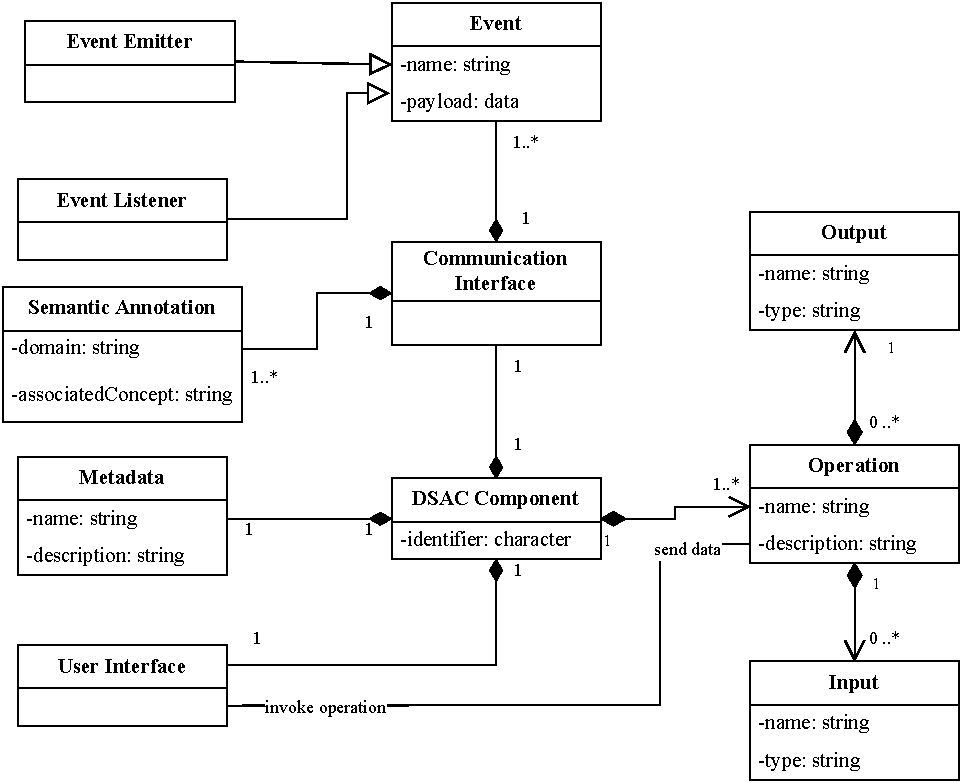
\includegraphics[width=0.85\textwidth]{../figures/MyFigures/ComponentModel.drawio.pdf}
\captionsetup{justification=centering}
\caption{\gls{dsac} Component Model}\label{fig:component-model}
}
\end{figure}

\begin{thesisdefinition}{Component Model}{def:component-model-formalism}

In \gls{dsac} a Component \(C\) is a 5-tuple of metadata, \gls{dom} elements, set of operations, number of event handlers and listeners as communication interface, and semantic annotations defined as:
\begin{equation}\mathfrak{C} = <M,UI,OP,CI,SA>\label{eq:component-tuple}\end{equation}
\end{thesisdefinition}

\vspace{-5pt}
\textbf{Component Metadata} as 	\(M = < name,\ description >\) consists of the name and component's functionality description. The metadata is important during the discovery phase.

\textbf{User Interface} denoted as \(UI\) enables the domain expert's interaction with the component. The UI is represented as a node in the \gls{dom} tree that allows users to initiate actions to prompt the component to execute tasks or alter its state.

\textbf{Component Operations} denotes as
\(OP = \  < name,\ description >\) and has multiple Input and Output, where:

\begin{itemize}
\item
\(I = < name,\ type >\) represents the operation input.
\item
\(O = < name,\ type > \ \ \)represent the operation output.
\end{itemize}

\textbf{Communication Interface \(CI\)} as \( \ < Evt,EvtEmitter,\ EvtListener >\), where:
\begin{itemize}
\item
Event:\(\ Evt = \{ E_{n} = < name,payload > \}\) where each event
\(e_{n}\) has a unique name (identifier) and associated data as
  payload. The payload data is produced by \(EvtEmitter\) and consumed
  by \(EvtListener\).
\item
  The \(EvtEmitter = \{{ee}_{i}|\ {ee}_{i}\  \in Evt\}\) is a set of
  event emitter functions supported by the component. The \(EvtEmitter\)
  fires events as a result of performing an action or state change ,
  triggering the invocation of a registered event listener for the
  corresponding event.
\item
  The \(EvtListener = \{{el}_{i}|\ {el}_{i}\  \in Evt\}\) is a set of
  event listener functions supported by the component. These listeners
  respond to events triggered by the event emitters.
\end{itemize}

\textbf{Semantic Annotation} as \(SA = \  < Domain,\ AssociatedComponet >\) consists of Domain,
representing the domain of the component and Associated Concept, to link
the component with the ontology concepts using their \gls{iri}.

 
\vspace{-20pt}
\hypertarget{sec:Composition-model}{%
\subsection{Composition Model}\label{sec:Composition-model}}
\vspace{5pt}

Composition involves linking the events (or responses) emitted by one
component with the operation invocations of another component. The data
flow among components is determined by the component’s communication
interface. The component’s choreography and the template
for the final result mashup are established by the platform-independent
composition model \autocite{Daniel2009d}. This model covers
various aspects of the solution, including the involved components,
communication medium, as well as the \gls{ui} layout and its behavior. In other
words, the composition model acts as a template for component
orchestration, aligning with the domain experts’ goals
\autocite{Pietschmann2010}.
The \cref{fig:composition-model} illustrate the composition model.
\begin{figure}[hbt]
\hypertarget{fig:composition-model}{%
\centering
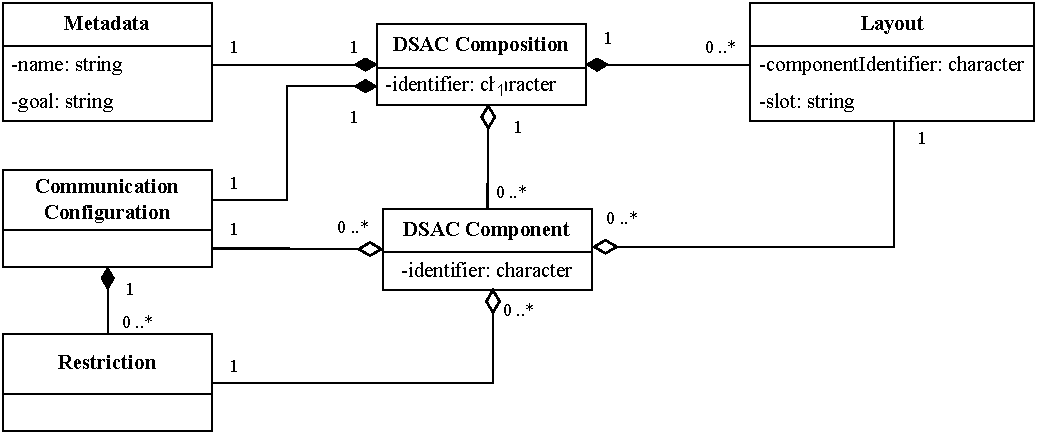
\includegraphics[width=0.85\textwidth]{../figures/MyFigures/CompositionModel.drawio.pdf}
\captionsetup{justification=centering}
\caption{\gls{dsac} Composition Model}\label{fig:composition-model}
}
\end{figure}

\begin{thesisdefinition}{Composition Model }{def:composition-model-formalism}

Composition Model \(CM\) is a 4-tuple of metadata, layout, component list, and component's communication channels defined as:
\begin{equation}\mathfrak{CM} = <M,L,CE,CC>\label{eq:composition-tuple}\end{equation}
\end{thesisdefinition}

\textbf{Composition Metadata} as 	\(M = < name,\ goal >\) 	>, consists of \emph{name} and \emph{goal} envisioned by the domain expert to be achieved through the end application.
\textbf{Layout Model} as \(L = \ {\{ c}_{i},\ Slot\}\), where \(,\ Slot\) represents the placeholder for each component \(c_{i}\) within the \gls{ui} model.
\textbf{Communication Configuration} as \emph{}\(\ CC = (V,\ E,\ R)\) defining the communication channels among components. Theconfiguration is represented as a graph, where:

  \begin{itemize}
  \item
    \(V\) denotes the vertices representing the components.
  \item
    \(E\) denotes the edges, representing communication paths between
    two components. There is a communication path among \(c_{i}\ \)and
    \(c_{j}\ \)if:
    \[c_{i}.O \subseteq c_{j}.I\  \cup \ c_{i}.I\  \supseteq c_{j}.O\]  
  \item 
 \( R = \{ r_{i} \mid r_{i} = \langle c_{i}, c_{j} \rangle \} \) denotes set of
    restriction on component coupling.
  \end{itemize}
  
The inter-component communication paradigm, as defined in this composition model, is based on an event-based architecture, which is inherently supported by the component model’s design. 
  
\vspace{-10pt}
\hypertarget{sec:process-model}{%
\subsection{Process Model}\label{sec:process-model}}
\vspace{10pt}
In software engineering, the process model represents the development process abstraction. To enhance the solution efficiency and avoid potential implications in early phases, the process model should include the phases, artifacts, and users’ roles \autocite{Yu1994}. In line with the principle of ‘Segregation of Responsibilities’, the process model should clearly define the different logical roles involved in the development process based on their level of expertise from domain and technical aspect. Involved roles are illustrated in \cref{fig:role-model}:
\begin{figure}[hbt]
\hypertarget{fig:role-model}{%
\centering
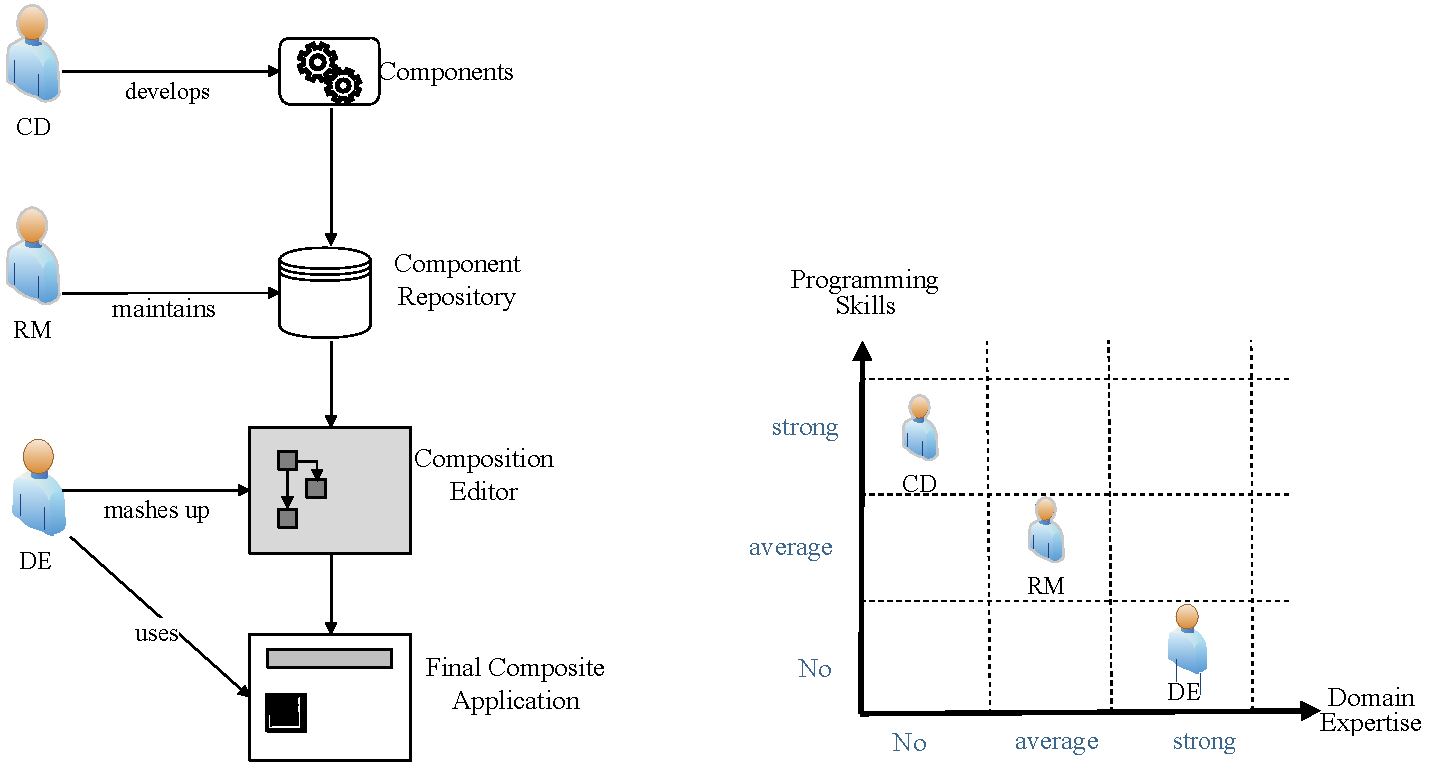
\includegraphics[width=0.85\textwidth]{../figures/MyFigures/roles.drawio copy.pdf}
\captionsetup{justification=centering}
\caption{\gls{dsac} Role Model}\label{fig:role-model}
}
\end{figure}

\textbf{\gls{cd}}are skilled programmers responsible
for supervising the semi-automatic component generation process. Each
component encapsulates a specific service, which can be glued together
to address complex problems. Supervising the component generation
process requires specific programming skills, especially in the Web
Engineering domain.

\textbf{\gls{rm}} maintains the public or private
component repository and oversees the component documentation to promote
reusability and enhanced discovery. Repository managers are domain
experts with average programming and domain knowledge.

\textbf{Domain Experts} are the decision-makers who have two roles in
\gls{dsac} process model. They serve as composition developers, developing
different mashup solutions by interacting with the mashup editor. Domain
experts are also the end users of the situational application for
decision making purposes. Domain experts can assume both roles
simultaneously or either one individually. In both cases, we assume that
domain experts have no technical expertise.

The \gls{dsac} is built upon the \gls{wcpm}
introduced in \autocite{Gaedke2000}. The process model in this work
is adopted from the spiral model, emphasizing a life-cycle- and
reusability-centric approach. The process is organized into two phases
covering the analysis, design, and implementation stages of web
application development.

As depicted in \cref{fig:process-model}, the process model consists of \emph{Initial
Phase} and \emph{Evolution Cycle}.During the Initial Phase, a
set of artifacts such as general-purpose components and the domain
knowledge base are generated. Domain Experts handle domain-specific data
preparation (\emph{Domain Analysis}). Subsequently, the domain ontology
is automatically generated under the supervision of domain experts
during the \emph{Knowledge Discovery} step. Furthermore, the Repository
Manager collects the \gls{api} specifications from online repositories and
organize them based on functionality and domain knowledge. Throughout
the \emph{Component Development} step, the general-purpose components
and template composition models are generated and stored in dedicated
repositories. The component developer also provides relevant metadata,
which is used during the component discovery and run-time composition
generation.

Focusing on the continuous evolution across the centralized reusable
repositories, the \emph{Evolution Cycle} includes iterative development
cycles, that divides the development process into three cyclic stages to
cover analysis, design, and implementation activities. The cycle starts
with, Initial Analysis, involves analyzing the user's query to identify
the target domain and goals as well as domain ontology generation and
implementation activities. The second step, \emph{Component Discovery}
involves a series of interactions with domain experts to identify the
desired functionalities and candidate components. The discovery
mechanism uses the component repository as a source of potential
candidates. Repository Manager is responsible for making the potential
components available for composition. According to the list of candidate
components, the potential composition paths are generated and integrated
into the composition model.

\begin{figure}[hbt]
\hypertarget{fig:process-model}{%
\centering
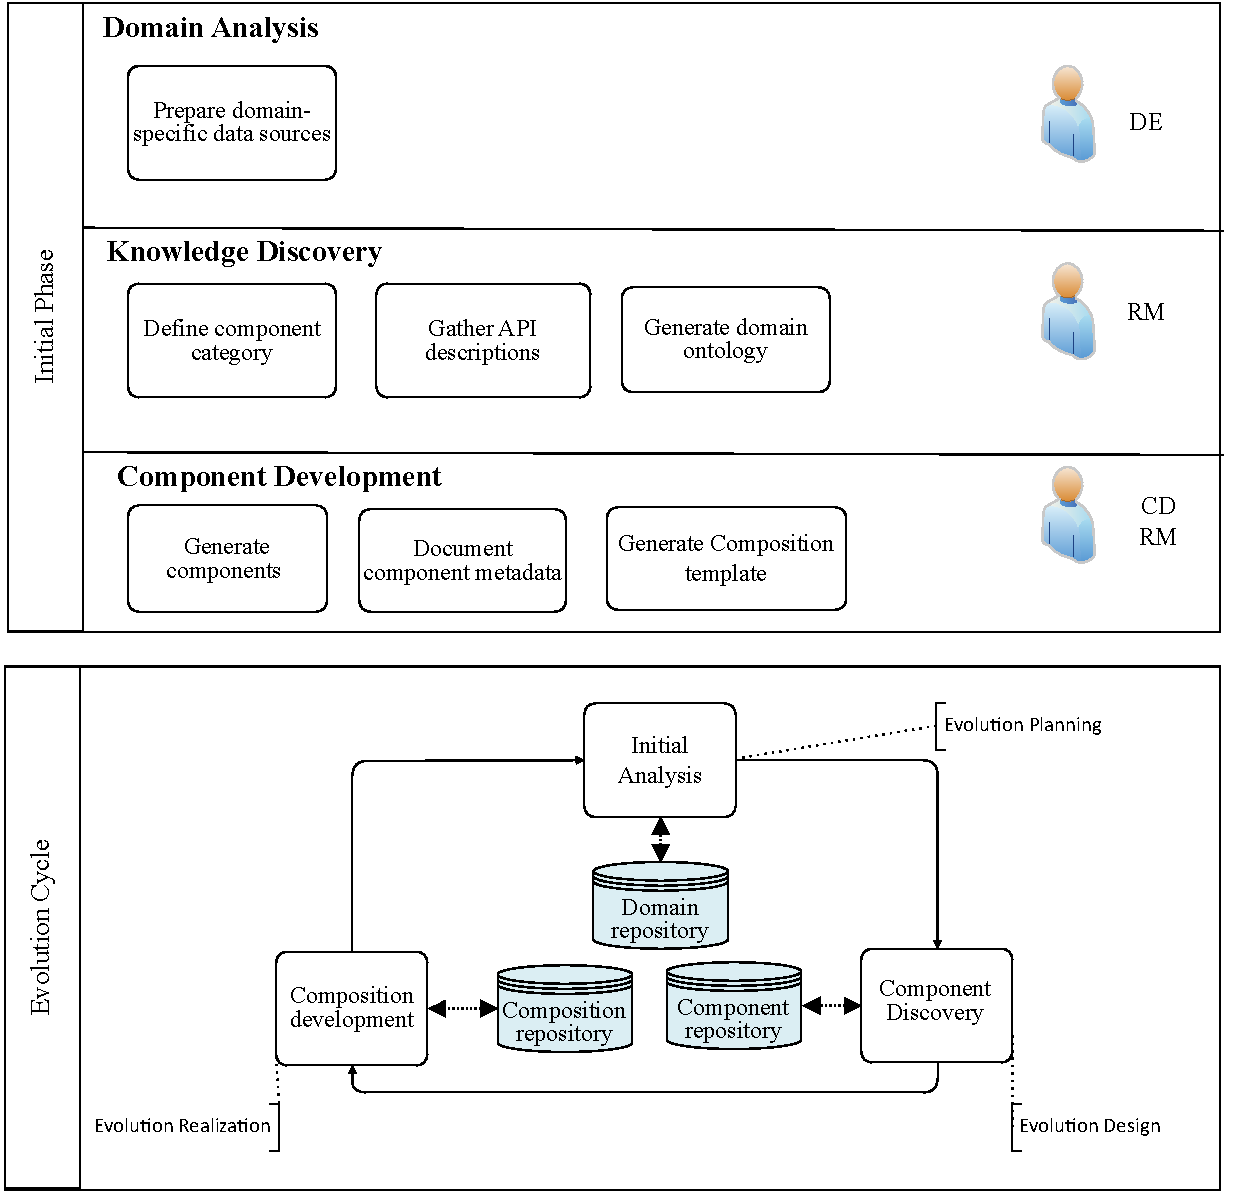
\includegraphics[width=0.85\textwidth]{../figures/MyFigures/PM.drawio.pdf}
\captionsetup{justification=centering}
\caption{\gls{dsac} process Model}\label{fig:process-model}
}
\end{figure}
The evolution process can start with an empty solution template if no existing solution is found. In accordance with the ‘Promote Reusability’ principle, the Repository Manager archives the reusable solutions as the composition template for other use cases. The components are similarly stored in the component repository, ensuring their availability for future use.

\vspace{-10pt}
\hypertarget{sec:tools}{%
\section{Tools and Methods}\label{sec:tools}}
\vspace{10pt}

This section introduces three Methods as primary applied techniques during development phases. Each method addresses one of the research objectives and provide necessary techniques and tools to solve the identified problems in \cref{sec:problem}.
\begin{itemize}
  \item
  Model-driven Composition Development
  \item
  Conversational-based Discovery and Composition Technique
  \item
  Ontology-based Platform Development 
  \end{itemize}
The overview of methods and related tools in each phase is depicted in \cref{fig:methods}.

\begin{figure}[hbt]
\hypertarget{fig:methods}{%
\centering
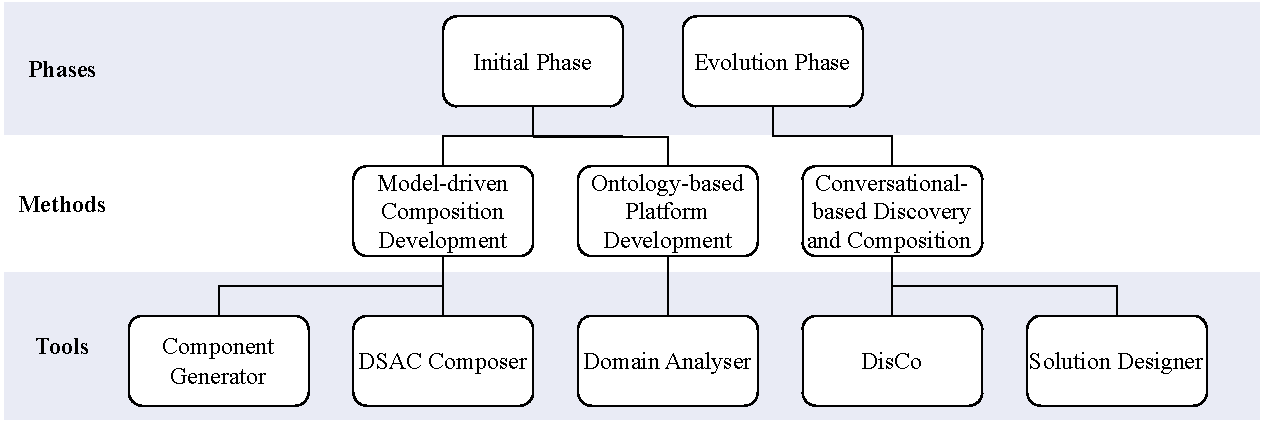
\includegraphics[width=0.85\textwidth]{../figures/MyFigures/Methods.drawio.pdf}
\captionsetup{justification=centering}
\caption{\gls{dsac} Methods and Toolkit}\label{fig:methods}
}
\end{figure}

\vspace{-18pt}
\hypertarget{sec:mdcd}{%
\subsection{Model-Driven Composition Development}\label{sec:mdcd}}
\vspace{4pt}
This method addresses the usability subproblem outlined in \cref{sec:problem} by facilitating the development of an easy-to-use composition platform. This method involves a series of model transformations to generate the model-compliant components in a time and cost-efficient manner. In accordance with the "Promote Reusability" principle, existing \gls{api}s are encapsulated conforming to the defined component model (cf. \cref{sec:component-model}). Subsequently, these components are configured and integrated within the composition model, resulting the final composite platform. Following the "Abstraction Slop" principle, these steps are easily navigable for non-technical users, ensuring a smooth slope of difficulty.
Generating the model-driven composition platform is supported by the two following tools.

The \textbf{Component Generator }(cf. \cref{sec:component-gen}) is tasked with generating executable \gls{dsac} components according to the \gls{api}’s specifications. The generated component is conformed to the defined component’s metamodel. This tool automates the first step in composition platform generation to enhance the platform's usability. The component generator maps the \gls{api}’s data schema and structure within component and generate the executable client code.

The \textbf{\gls{dsac} Composer} (cf. \cref{sec:dsac-composer}) configures and instantiates the composition model. Once the model is generated, the Composition Compiler compiles executable code and generates the run time environment. To ensure the domain specificity, the run time environment adjusts its behavior based on domain specifications provided by the Domain Analyzer. This approach will guarantee the proper application of the "Domain Focused" principle.

\vspace{-15pt}
\hypertarget{sec:cbdiscovery}{%
\subsection{Conversational-Based Discovery}\label{sec:cbdiscovery}}
\vspace{4pt}

The method addresses the "Poor expressive power" discussed in \cref{sec:problem} and aligns with  (cf. \cref{ro:2}). By leveraging a conversational medium, Conversational-based Discovery provides a high level of expressive capability. Semantic interpretation techniques are employed to extract the business goals from the domain experts' utterances. Subsequently, the discovery mechanism retrieves the suitable components and possible composition solution to fulfill these goals. The conversational interface should provide an easy-to-use medium and reduce the possible errors during solution design. \cref{sec:dsac-discovery} presents tools implementing the Conversational-based Discovery and Composition Assistance through \gls{disco} and Solution Designer tools. 

\textbf{\gls{disco}} (cf. \cref{sec:disco}) supports domain experts by allowing them to retrieve the best-fitted components to achieve their goals. DisCo employs the Conversational-based Discovery technique, where domain experts engage in structured dialogues following a designed conversation flow. This tool facilitates the identification of the target domain and extraction of desired functionalities by leveraging the natural language as the interaction medium. The information extraction process continues until all the required data for instantiating the Request Template is collected. The Request Template, formatted in XML syntax, serves to retrieve components from the component repository. 

The \textbf{Solution Designer} (cf. \cref{sec:solution-Designer}) identifies the best composition paths for components according to the defined criteria. Once the potential components are discovered, the Solution Designer generates the Compatibility Graph as a directed weighted graph. The Compatibility Graph is considered as the communication interface of the composition model, determining the paths among the candidate components. Any change in the composition model and component selection will result in an updated solution graph.

\vspace{-15pt}
\hypertarget{sec:obpd}{%
\subsection{Ontology-Based Platform Development}\label{sec:obpd}}
\vspace{4pt}
This method addresses the domain specificity subproblem discussed in \cref{sec:problem} by utilizing formal ontologies during both the development and run time. Ontologies conceptualize domain knowledge using standards like \gls{owl} and \gls{rdf}, thereby forming a semantic layer. This layer differentiates between the \gls{dro}, which serves as the \gls{conceptual model} during development, and the \gls{doo}, which represents the business logic applied during run time. The run time environment adheres to domain-specific concepts and operations at component and composition levels.

This method is applied by the \textbf{Domain Analyzer} (cf. \cref{sec:onto.domain-analyser}) to generate the ontologies under domain experts’ supervision. The \gls{dro} represents the domain's terminology, key concepts, and terms, as well as the relationships between them, thereby providing a formal and semantically rich representation of domain knowledge. The \gls{doo}, which is derived from the \gls{dro}, contains the domain rules to be applied to composition model and \gls{ui}. By integrating the domain model into composition development, the composite application is endowed with enhanced intelligent decision-making capabilities.

\vspace{-12pt}
\section{Summary}
\vspace{13pt}

This chapter introduced the approach for developing a domain-specific situational application aimed at facilitating the decision-making process. Core concept of this approach is to provide methods to address the limitations of existing \gls{eud} approaches in tackling the usability and expressiveness challenges associated with situational applications. This method involves conceptual architectures of the component and composition models, the development process model, as well as methods and tools implementation. Moreover, a series of principles are presented to ensure the quality of final tool and the development process. These principles are domain focused design, abstraction slope, segregation of responsibilities and promoting reusability. The three methods in this chapter specify techniques for generating an easy-to-use model-driven composition application, enabling domain-specific customization, and enhancing expressiveness by enabling  natural language interaction. The implementation of these methods is proposed by tools. The next three chapters provide a detailed overview of each method and associated tool implementations.  